\documentclass[11pt, a4paper, titlepage]{article}
\setlength{\parindent}{0pt}

%%%%%%%% paquetes %%%%%%%%
%\usepackage[lmargin=2cm,rmargin=2cm,top=1.5cm,bottom=2cm]{geometry}
\usepackage[T1]{fontenc}
\usepackage[utf8]{inputenc}
\usepackage[spanish,es-tabla]{babel}
\usepackage{amsmath}
\usepackage{amssymb,amsfonts,latexsym,cancel}
\usepackage{fancyhdr}
\usepackage{titlesec}
\usepackage{titling}
\usepackage{anyfontsize}
\usepackage{color}
\usepackage[dvipsnames]{xcolor}

\usepackage{csquotes}   
\usepackage[style=numeric-comp, sorting=none, block=par]{biblatex} 
\DeclareFieldFormat{title}{\bfseries\emph{#1}}
\definecolor{softblack}{RGB}{74, 71, 71} 
\DeclareFieldFormat{howpublished}{\textcolor{softblack}{\mdseries{#1}}}
\DeclareFieldFormat{labelnumberwidth}{\mkbibbold{#1\adddot}}
\setlength\bibitemsep{2.5\itemsep}
\renewcommand*{\newunitpunct}{\addspace}
\renewcommand*{\finentrypunct}{\addspace}
\usepackage{listings}
\usepackage{graphicx}
\usepackage[colorlinks = true,
			linkcolor = black,
			urlcolor = black,
			citecolor = blue ]{hyperref}

%%%%%%%% encabezado y pie de página %%%%%%%%
%\pagestyle{fancy}
%\fancyhead{}
%\fancyfoot{}
%\fancyfoot[R]{\thepage}
%\fancyfoot[L]{2º Trabajo Optimización Heurística}
%\renewcommand{\headrulewidth}{0pt}

%%%%%%%% formato de títulos y subtítulos %%%%%%%%

\definecolor{gray75}{gray}{0.75}
\newcommand{\hsp}{\hspace{20pt}}
\titleformat{\section}[hang]{\huge\bfseries}{\thesection\hsp\textcolor{gray75}{|}\hsp}{0pt}{\huge\bfseries}
\titlespacing{\section}{0pt}{0pt}{15pt}
\titleformat{\subsection}[hang]{\Large\bfseries}{\thesubsection\hsp}{0pt}{\Large\bfseries}
\titlespacing{\subsection}{0pt}{35pt}{15pt}
\titleformat{\subsubsection}[hang]{\large\bfseries}{\thesubsubsection\hspace{10pt}}{0pt}{\large\bfseries} 
\titlespacing{\subsubsection}{0pt}{20pt}{0pt}

%\titleformat{\section}[block]{\LARGE\bfseries}{\thesection.}{1mm}{}
%\titlespacing{\section}{0pc}{5.5ex}{1pc}
%\titleformat{\subsection}[block]{\Large\bfseries}{\thesubsection.}{1mm}{}
%\titlespacing{\subsection}{1.5pc}{5.5ex}{1pc}



\begin{document}

	\begin{titlepage}
    	\begin{center}
        	\hrulefill

        	\vspace{0.5cm}
        	{\bf\fontsize{25}{0}{\selectfont{Optimización Heurística\\[0.5cm]}}}
        	\fontsize{15}{0}{\selectfont{Optimizar una calificación\\[0.5cm]}}
        	\hrulefill
        	\vspace{6.0cm}
    	\end{center}

    	\centering
    	{\Large Daniel Tomás Sánchez\\ Aarón Cabero Blanco \\ Pablo Bautista 				Frías \par}
    	\vspace{2cm}
    	{\Large 03/01/2020 \par}
	\end{titlepage}

\newpage

%\renewcommand{\contentsname}{\fontsize{22}{0}{\selectfont{Índice}}}
%{\Large \tableofcontents}

\tableofcontents

\newpage

\section{Introducción}
Durante la realización de esta práctica se ha planteado un problema de optimización para su posterior resolución. Se explicará en detalle el problema así como las operaciones realizadas para obtener la solución óptima con el algoritmo. Posteriormente se resolverá el problema con diferentes datos de entrada para así poder ver los distintos resultados obtenidos.

\newpage

\section{Descripción}
El problema planteado consiste en la optimización de la nota media obtenida en un conjunto de asignaturas por un alumno. Para que el caso sea lo más real posible, se han añadido distintas variables que afectan al resultado óptimo del problema, como por ejemplo, las horas de las que dispone el alumno para estudiar o la dificultad que tiene cada unas de las asignaturas.

\subsection{Variables del problema}
Las distintas variables usadas en el problema son:

\vspace{5mm}

\textbf{minimun\_marks (array)}: Esta variable representa la nota mínima que se puede sacar en cada asignatura. En caso de no sacar la nota mínima en una asignatura, no se podrá pasar con éxito el curso.

\vspace{5mm}

\textbf{point\_per\_hour (array)}: Cada elemento del array indica el número de horas que se deberá estudiar para sacar un punto en una asignatura. Esto también indica la dificultad de cada asignatura, cuantas más horas haya que estudiar para sacar un punto en una asignatura, mayor dificultad tendrá esta.

\vspace{5mm}

\textbf{credits (array)}: Indica el valor de cada asignatura mediante un sistema de créditos. Una asignatura con más créditos tendrá más valor que una con menos créditos, de esta forma, a la hora de hacer la media, ponderará más una asignatura con más créditos.

\vspace{5mm}

\textbf{revision\_probability (array)}: Mediante esta variable se indica la probabilidad que tiene una asignatura de que en la revisión se le suba nota al alumno. Dado que esta variable se combina con ''studen\_luck'' para determinar si finalmente al alumno se le subirá la nota, cuanto menor sea el número en ''studen\_luck'' más fácil será para el alumno subir nota en dicha asignatura. Los elementos del array deberán estar entre los valores 0 y 1.

\vspace{5mm}

\textbf{studen\_luck (array)}: Tal y como hemos mencionado anteriormente, esta variable se combina con la anterior para determinar si un alumno subirá nota en una asignatura o no. Si ''studen\_luck'' es menor o igual que ''revision\_probability'', el alumno subirá nota en dicha asignatura. Los elementos del array deberán estar entre los valores 0 y 1.

\vspace{5mm}

\textbf{revision\_mark (array)}: En el caso de que, según lo anterior, el alumno suba nota en una asignatura, ''revision\_mark'' indica la puntuación que subirá dicho alumno en la asignatura. Dado que las asignaturas se califican con una puntuación entre 0 y 10, un alumno nunca pondrá obtener una nota superior a 10 tras realizar la revisión. Para no variar demasiado los resultados obtenidos en las asignaturas, los valores entre los que se comprenden los elementos del array se encontrarán entre 0 y 0.5.

\vspace{5mm}

\textbf{study\_hours (int)}: La variable ''study\_hours'' representa el número total de horas de las que dispone un alumno para estudiar. El resultado óptimo no pondrá tener un número total de horas mayor que las horas de las que dispone el alumno.

\vspace{5mm}

Todas las variables anteriores se encuentran dentro del fichero ''Data.py'' y pueden ser modificadas. A la hora de modificar estas variables hay que tener en cuenta que el tamaño de los arrays debe ser el mismo, y este tamaño será igual al número de asignaturas con las que queramos plantear el problema. Además de las variables anteriores, existen otras variables que se introducirán por terminal, o que en su defecto, tendrán valores predeterminados. Estas variables son las siguientes: 

\vspace{5mm}

\textbf{population\_size (int)}: Esta variable indica el tamaño de la población, en los casos donde no se introduzca mediante la terminal, su valor predeterminado será de 50.

\vspace{5mm}

\textbf{iterations (int)}: Esta variable indica el número de iteraciones que se realizará el algoritmo, al igual que la anterior, en los casos en los que no se introduzca por la terminal tendrá un valor predeterminado, y este valor será de 500.

\vspace{5mm}

\textbf{reps (int)}: Indica el número de repeticiones que se realizará el algoritmo. Esta variable será obligatoria introducirla en los casos en los que se pida.

\subsection{Bounds}

En el problema que estamos tratando, el rango de los valores de los posibles candidatos puede variar dependiendo de los valores que obtengan las variables de entrada. Aún así, el rango de valores una vez se han introducido las variables de entrada se obtiene según la siguiente fórmula matemática:
\[
(minimum\_marks[i] / point\_per\_hour[i], 10 / point\_per\_hour[i])
\]

De esta forma, el rango irá desde las horas que necesita un alumno para sacar la nota mínima, a las horas que necesita un alumno estudiar para sacar un 10, que es la máxima nota.

\newpage

\section{Función Fitness}
Dado que nuestro problema consiste en maximizar la nota del alumno, cuanto mayor sea el ''fitness'' mejor será el resultado. A continuación mostraremos la parte del código utilizada para el ''fitness'' y posteriormente procederemos a explicarla.

\vspace{5mm}

\textcolor{orange}{def} \textcolor{yellow}{our\_fitness}(array):\\\hspace*{1em} res = \textcolor{blue}{0}\\
\hspace*{1em} \textcolor{orange}{for} i \textcolor{orange}{in} \textcolor{blue}{range}(\textcolor{blue}{len}(array)):\\
\hspace*{2em} mark = (array[i] * point\_per\_hour[i])\\
\hspace*{2em} \textcolor{orange}{if} student\_luck[i] <= revision\_probability[i]:\\
\hspace*{3em} mark += revision\_mark[i]\\
\hspace*{2em} \textcolor{orange}{if} mark > \textcolor{blue}{10}:\\
\hspace*{3em} mark = \textcolor{blue}{10}\\
\hspace*{2em} res += mark * credits[i]\\
\hspace*{1em} nota = res / \textcolor{blue}{sum}(credits)\\
\hspace*{1em} \textcolor{orange}{if} \textcolor{blue}{sum}(array) > study\_hours:\\
\hspace*{2em} return -((\textcolor{blue}{sum}(array) - study\_hours) ** \textcolor{blue}{2} / nota)\\
\hspace*{1em} \textcolor{orange}{return} nota\\

\vspace{5mm}

La función ''fitness'' se encarga de calcular la nota media obtenida por el alumno. En primer lugar, se calcula la nota que sacaría en cada una de las asignaturas, multiplicando las horas que dedica a esa asignatura por los puntos que se obtienen en dicha asignatura por cada hora estudiada ($ array[i] * point\_per\_hour[i] $). Una vez que el alumno obtiene la nota de la asignatura, tal y como hemos mencionado anteriormente, cabe la posibilidad de subir nota en la revisión. Si la suerte del estudiante en esa asignatura es menor que la probabilidad de revisión de esa misma asignatura ( $ student\_luck[i] <= revision\_probability[i] $ ), el alumno recibirá una subida de nota igual a la cantidad que el array ''revision\_mark'' tenga en la posición en la que se encuentra la asignatura ( $ mark += revision\_mark[i] $ ). En caso de que tras la subida de nota, la calificación del alumno fuese mayor de 10 puntos ( $ mark > 10 $ ), dicho alumno se quedaría con una nota igual a 10 ( $ mark = 10 $ ). Posteriormente se guardará el valor que le ha otorgado esa nota al alumno en la variable ''res'', realizando la multiplicación de dicha nota por los créditos de la asignatura ( $ res += mark * credits[i] $ ) dado que una asignatura con más créditos tendrá más peso en la nota final. Para finalizar, se realizará la media con todos los resultados, esto se hace dividiendo el resultado final que hemos obtenido en ''res'' por los créditos totales de las asignaturas ( $ nota = res / sum(credits) $ ) y el resultado de esa nota será lo que devuelva nuestra función ''fitness''.

\vspace{5mm}

En el caso de habernos pasado de horas de estudio, es decir, que las horas de estudio que hemos empleado sea mayor que el número de horas de estudio de las que disponía el alumno ( $sum(array) > study\_hours$ ), el resultado será un valor negativo ( $ -((sum(array) - study\_hours) ** 2 / nota)$ ). De esta forma guiaremos al algoritmo al resultado más optimo sin sobrepasar las horas de estudio de las que el alumno dispone.
        
\newpage



\section{Ejemplos}
A continuación, vamos a realizar algunos ejemplos para visualizar los resultados obtenidos con el algoritmo y como se visualizan estos.

\subsection{Horas insuficientes para aprobar}
En este primer ejemplo, el número de horas de las que dispone el alumno, es inferior a las horas mínimas necesarias para sacar la nota mínima en todas las asignaturas, lo que implica que el alumno no podrá aprobar el curso. Vamos a ver como se comporta el algoritmo en esta situación.

\vspace{5mm}

\begin{itemize}
\item \textbf{Variables de entrada}
\end{itemize}
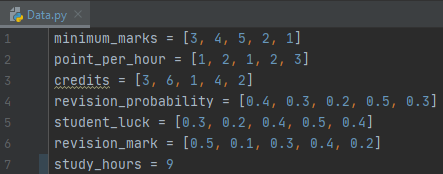
\includegraphics[scale=1]{img/Data_horas_insuficientes.png}

\subsubsection{Resultados con 1 repetición}
Los resultados obtenidos al realizar una repetición del algoritmo son los siguientes:

\vspace{5mm}

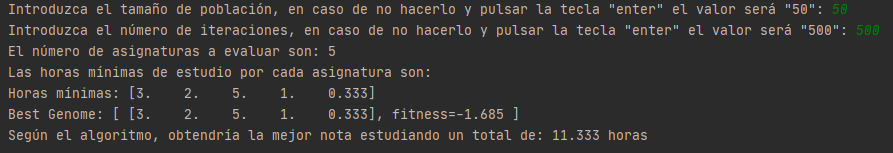
\includegraphics[scale=0.7]{img/Res1_horas_insuf.png}

\vspace{5mm}

Como se puede observar en la imagen del resultado, el ''fitness'' obtenido es un número negativo. Esto sucede debido al ejemplo en el que nos encontramos, donde el número de horas de las que dispone el alumno es insuficiente para llegar a la nota mínima de todas las asignaturas.

\vspace{5mm}

Esto también podemos observarlo en el vector ''Horas mínimas'' donde nos indica las horas que deberíamos estudiar cada asignatura para llegar a su nota mínima y cuyo sumatorio es igual a 11.33, un número de horas mayor de las que dispone el alumno en el ejemplo (study\_hour), que son 9 horas (tal y como se puede observar en la imagen de ''Variables de entrada'').


\subsubsection{Resultados con varias repeticiones}
Ahora realizaremos varias repeticiones del mismo ejemplo para ver gráficamente las diferencias entre los distintos resultados. En esta ocasión, el número de repeticiones que realizaremos serán 10, pero estas repeticiones pueden introducirse en cada ejemplo mediante la terminal.

\vspace{5mm}

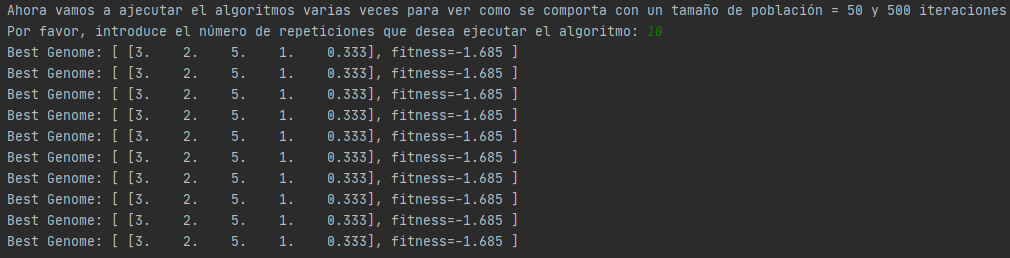
\includegraphics[scale=0.6]{img/Res2_horas_insuf.png}

\vspace{5mm}

En la imagen, podemos observar como todos los resultados coinciden con las horas mínimas de estudio para cada asignatura, esto sucede porque el alumno no dispone de horas suficientes para alcanzar la nota mínima, por lo que no podría aprobar el curso con éxito, de ahí que todos los ''fitness'' resultados sean negativos.

\vspace{5mm}

Ahora visualizaremos el resultado de los distintos ''fitness'' mediante diagramas de cajas, para así tener una imagen más visual de los resultados que se han obtenido.

\newpage

\begin{itemize}
\item \textbf{Mejor fitness de cada repetición}
\end{itemize}

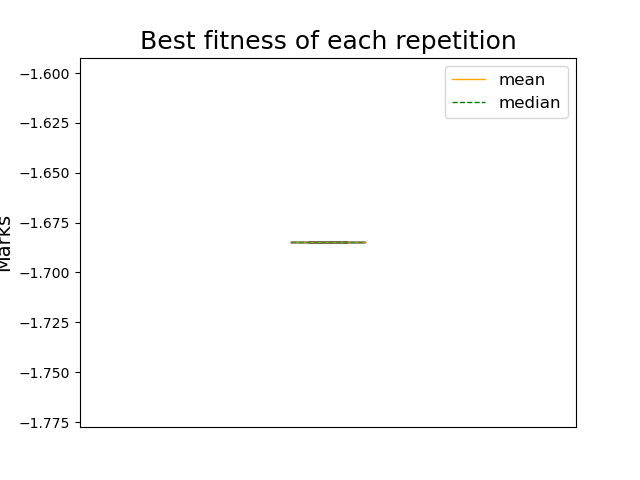
\includegraphics[scale=0.6]{img/grafica1_horinsuf}


En el gráfico podemos ver representado el resultado de la imagen anterior, en el que el mejor fitness de cada repetición es -1.685. Dado que todos los mejores fitness de cada repetición tienen el mismo valor, en este caso no podemos apreciar el diagrama de caja, pero si podemos apreciar que el resultado obtenido en el diagrama es el correcto.

\vspace{5mm}

\begin{itemize}
\item \textbf{Todos los fitness de cada repetición}
\end{itemize}

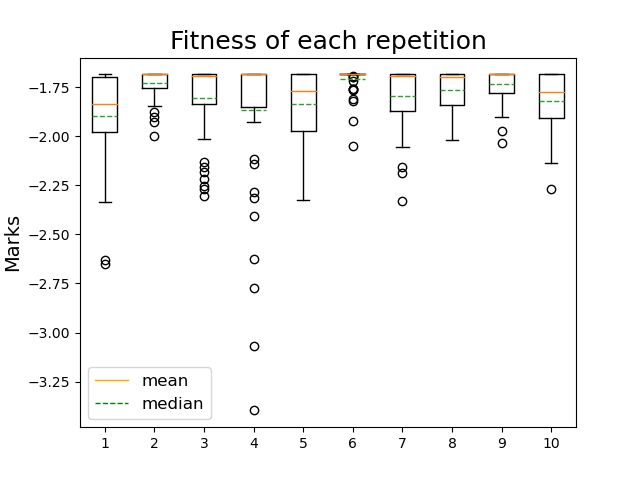
\includegraphics[scale=0.6]{img/grafica2_horinsuf}

Este diagrama nos muestra todos los fitness que se han obtenido por cada una de las 10 repeticiones. Dado que las horas de estudio del alumno son inferiores a las horas mínimas necesarias para sacar la nota mínima de cada asignatura, todos los resultados obtenidos son resultados negativos, además de obtener muchos resultados dispares. Como podemos observar en el diagrama de caja, existen muchos resultados atípicos debido a la naturaleza del ejemplo en el que nos encontramos.

\subsection{Horas suficientes para aprobar}
Este ejemplo plantea un escenario totalmente distinto al anterior. En esta ocasión, el alumno dispondrá de las horas suficientes para poder sacar la nota mínima en todas las asignaturas, y partiendo de este punto, veremos cuantas horas debe dedicar a cada una de las asignaturas para sacar la mayor nota posible en el curso. El ejemplo se realizará con las mismas variables de entrada que el ejemplo anterior, pero aumentando el número de horas de estudio (study\_hour) a 16.

\vspace{5mm}

\begin{itemize}
\item \textbf{Variables de entrada}
\end{itemize}
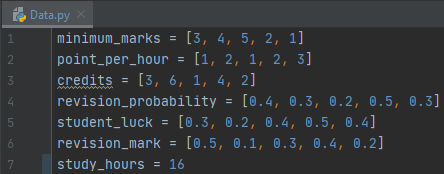
\includegraphics[scale=1]{img/Data_horas_sufi.png}

\subsubsection{Resultados con 1 repetición}
Los resultados obtenidos al realizar una repetición del algoritmo son los siguientes:

\vspace{5mm}

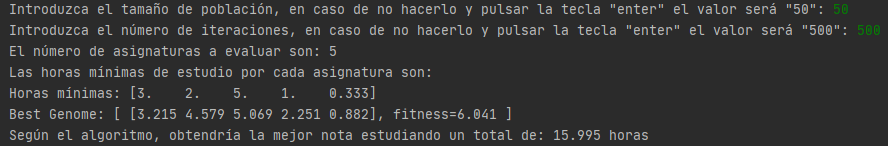
\includegraphics[scale=0.7]{img/Res1_horas_sufi.png}

\vspace{5mm}

En los resultados se pueden observar varias cosas, por un lado, al igual que en el ejemplo anterior, nos muestra un vector con las horas mínimas de estudio necesarias para alcanzar la nota mínima en cada asignatura (Horas mínimas), y por otro lado nos muestra las horas optimizadas para cada asignatura (Best Genome) de tal forma que podamos alcanzar la nota máxima con las horas de estudio disponibles que tenemos (16).

\vspace{5mm}

El fitness obtenido es 6.041, según el algoritmo, esta sería nuestra nota en caso de dedicar las hora obtenidas en ''Best Genome'' a cada una de las asignaturas, lo cual serían un total de 15.995 horas (aproximadamente las 16 horas de entrada).



\subsubsection{Resultados con varias repeticiones}
En este apartado se realizarán 10 repeticiones del algoritmo para el mismo ejemplo. De esta forma podremos observar como se comporta el algoritmo al realizar varias repeticiones y como varían los resultados entre las distintas repeticiones.

\vspace{5mm}

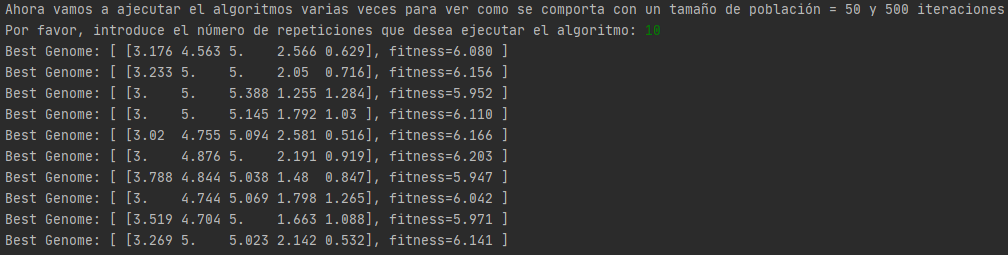
\includegraphics[scale=0.6]{img/Res2_horas_sufi.png}

\vspace{5mm}

Aquí podemos observar los resultados de cada una de las 10 iteraciones. Como se puede ver en la imagen, no hay gran diferencia entre los ''fitness'' de cada repetición, lo que indica que el algoritmo funciona correctamente. En este ejemplo, el 'fitness'' lo podemos encontrar entre los valores 5.9 y 6.2, pero eso se podrá observar mejor en los diagramas de cajas a continuación. 

\newpage

\begin{itemize}
\item \textbf{Mejor fitness de cada repetición}
\end{itemize}

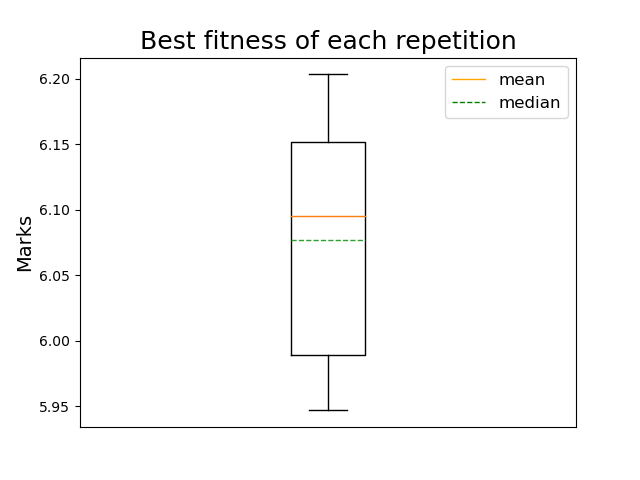
\includegraphics[scale=0.6]{img/grafica1_horsuf}

\vspace{5mm}

Tal y como hemos mencionado antes, en este diagrama de cajas se puede apreciar con más claridad el rango en el que se encuentra el ''fitness'' de cada una de las repeticiones. La media la podemos encontrar aproximadamente en el valor 6.1.

\vspace{5mm}

Por otro lado, podemos observar como el mejor ''fitness'' de las 10 repeticiones se encuentra en el valor 6.2, lo que nos indicaría que tras realizar varias veces el algoritmo, la nota máxima que podemos alcanzar con 16 horas de estudio es 6.2 si las distribuimos de la siguiente forma: [3.    4.876 5.    2.191 0.919] ocupando cada posición del vector una asignatura.

\newpage

\begin{itemize}
\item \textbf{Todos los fitness de cada repetición}
\end{itemize}

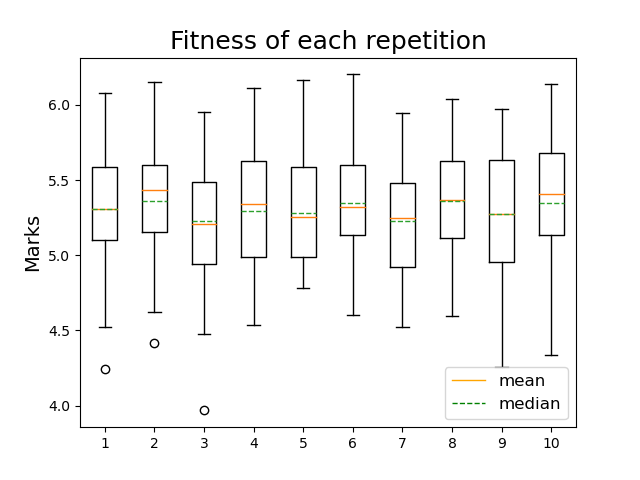
\includegraphics[scale=0.6]{img/grafica2_horsuf}

\vspace{5mm}

En este segundo diagrama de cajas podemos observar los valores ''fitness'' que se han ido obteniendo en cada una de las repeticiones. Podemos observar como la distribución de los datos obtenidos en cada una de las repeticiones es muy similar, exceptuando algunos datos que se encuentran separados, los cuales podríamos tomar como anomalías.

\vspace{5mm}

En este diagrama se observa mejor el funcionamiento del algoritmo que en el ejemplo anterior, ya que el alumno dispone de las horas suficientes para estudiar todas las asignaturas y alcanzar la nota mínima, el programa puede optimizar las horas para encontrar el resultado con el cual el alumno se acercará a la mejor nota, y esto se ve reflejado en la distribución de los datos obtenidos.

\newpage

\section{Conclusiones}
Este trabajo nos ha ayudado a afianzar los conocimientos obtenidos durante la asignatura. La ocasión de plantear nosotros mismos un problema, y más en este caso donde el problema nos toca tan de cerca, nos ha ayudado a poder seguir el proceso lógico del algoritmo con más facilidad.

\vspace{5mm}

También nos ha brindado la oportunidad de poder jugar con las variables de entrada y distintos valores, para ver de esta forma como se alteraban los resultados y comprender mejor el funcionamiento.

\vspace{5mm}

Por último, no solo nos ha servido para aprender, si no que al ser un ejemplo muy visual y como hemos mencionado anteriormente, un ejemplo cercano a nuestra situación, nos ha resultado curioso probar distintas variaciones para alterar de esta forma los resultados e imaginarnos como sería aplicar este problema a nuestro día a día en la facultad.

\end{document}